\documentclass[12pt]{article}

\usepackage[english]{babel}
\usepackage[utf8]{inputenc}
\usepackage[T1]{fontenc}
\usepackage{graphicx}
\usepackage{amsmath}
\usepackage{fancyhdr}
\usepackage{siunitx}
\usepackage{listings}

\makeatletter
\def\@seccntformat#1{\csname the#1\endcsname\hspace*{0.5em}$|$\hspace*{0.5em}}
\makeatother

\pagestyle{fancy}

\title{\textbf{Quartz resonator} \\ SCI-C0200}
\author{Joonatan Bergholm 507260 \\ Osama Abuzaid 524832}

\begin{document}

\pagenumbering{gobble}
\maketitle
\newpage

\pagenumbering{arabic}

\tableofcontents
\newpage

\section{Introduction}

In this assignment we investigated electronic properties of one of the most common electronic components, the quartz tuning fork or quartz resonator, like one in figure \ref{fig:kvres}. It is used in watches and other every day electrical appliances to provide a stable clocking frequency. Typically the frequency is $f_0 = \SI{32768}{\hertz}$, because is is a round number ($32768_{10} = {2^{15}}_{10} = 1000000000000000_2$) in base 2, which is commonly used in electrical appliances.

Contrary to conventional tuning fork, one does not need generate mechanical excitation
on the quartz tuning fork, because quartz has piezoelectric properties and thus mechanical excitation can be replaced with electronic one.

\section{Tuning fork}
Piezoelectricity is a phenomena, where deformation of a material causes electrical current and vice versa. Crystal oscillators are made of piezoelectric materials, and in electric circuits they are used to produce an electrical signal with precise frequency. The Q-value of crystal oscillator is defined to be the oscillators energy per dissipated energy at one oscillation:
\begin{align}
Q \equiv 2\pi\frac{E}{\Delta E}.
\end{align}

In our work we are using quartz tuning forks. The fundamental frequency of a tuning fork is given by equation
\begin{align}
f_0 \approx 0.16\frac{T}{L^2}\sqrt{\frac{E}{\rho}},
\end{align}
where $L = 3.98 $mm is the length of one quartz bar, $T = 0.60 $mm the width of the bar, $E = 79 $GPa the Young modulus and $\rho = 2660\frac{\mathrm{kg}}{\mathrm{m}^3}$ the density of quartz. Also the thickness of fork we are using in our work is $H = 0.30$mm. Advantage of having two bars instead of one is that the oscillations of two bars at the fulcrum cancel each other, resulting to better Q-value.

We can estimate the Q-value of the tuning fork from figure \ref{fig:steady} by using equation$^{\cite{Qvalue}}$
\begin{align*}
t &= \frac{f_0}{Q}\\
\Rightarrow Q &= tf_0 \approx 13000
\end{align*}
where $t \approx 0.4$s is the time constant, which tells the time it takes for the resonator to stabilize to the equilibrium amplitude.

\begin{figure}
\centering
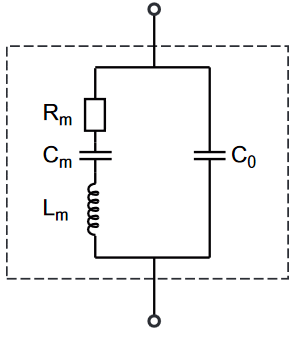
\includegraphics[width = 0.5\textwidth]{equivalence_circuit}
\caption{Equivalence circuit of a tuning fork.} \label{fig:equivalence_circuit}
\end{figure}

An equivalence circuit of tuning fork is an electrical circuit which can't be distinguished from tuning fork in a black box. The components of equivalence circuit in figure \ref{fig:equivalence_circuit} are obtained from following equations:
\begin{align}
\begin{cases}
L_m = \frac{2\rho L^3}{9e_p^2HT}\\
C_m = \frac{1}{\omega_0^2L_m}\\
R_m = \frac{\omega_0 L_m}{Q}=\gamma L_m\\
C_0 = \frac{\epsilon_0\epsilon_rA}{T}
\end{cases},
\end{align}
where $e_p \approx 0.18 \frac{\mathrm{C}}{\mathrm{m}^2}$ is the piezoelectric modulus of tuning fork, $\epsilon_0$ and $\epsilon_r$ are the vacuum and relative permittivity, respectively, and $A = TL$ the effective area. Equivalence circuit of our tuning fork would have following components:
\begin{align*}
\begin{cases}
L_m \approx 3.3\cdot10^{-20}~\mathrm{H}\\
C_m \approx 7.1\cdot10^8~\mathrm{F}\\
R_m \approx 5.3\cdot10^{-19}~\Omega\\
C_0 \approx 3.5\cdot10^{-9}~\mathrm{F}
\end{cases}.
\end{align*}

As we can see, the values are far from typical, so it would be very difficult and expensive to produce needed components.

\section{Measurement methods}
To collect data we used a DAQ (Measurement Computing USB-1208HS-2AO analog input/output device). We used its analog out -function to produce wanted signals to the circuit in figure \ref{fig:circuit} and collected both it's original signal and the modified signals with analog inputs. The triangle in the circuit represents an operation amplifier, which transforms $V_+$ and $V_-$ signals to a single signal $V_{out}$:

\begin{align}
	V_{out} = A(V_+-V_-).
\end{align}
$A$ is a very large number, so in practice $A_{out}$ can get only values 9V and -9V.

The whole circuit works as a voltage amplifier. Calculations are in appendix \ref{sec:voltamp}, and the final result is
\begin{align}
V_{out} = -\frac{R_F}{R_1}V_{in}.
\end{align}

\begin{figure}
	\centering
	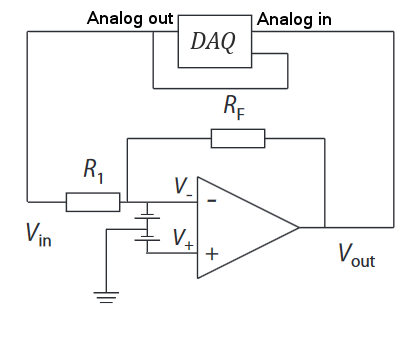
\includegraphics[width = 0.5\textwidth]{kuvat/piiri}
	\caption{Circuit used to collect data. Both batteries are 9V.}
	\label{fig:circuit}
\end{figure}

\begin{figure}
	\centering
	\includegraphics[width = \textwidth]{kuvat/kvres.png}
	\caption{Quartz resonator}
	\label{fig:kvres}
\end{figure}

\section{Results}

\begin{figure}
	\centering
	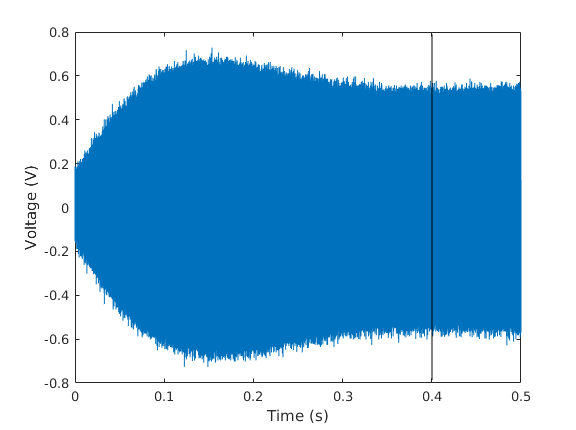
\includegraphics[width = \textwidth]{kuvat/steadystate.png}
	\caption{Steady state}
	\label{fig:steady}
\end{figure}

\begin{thebibliography}{1}
\bibitem{Qvalue} \texttt{https://mycourses.aalto.fi/pluginfile.php/211810/mod\_resource/content/1\\/projekti\_kertaohje4.pdf}, "Kvartsiresonaattorin mittaus", accessed 2016.06.01
\end{thebibliography}

\appendix

\section{Source code}

\lstinputlisting[caption = ac.m]{matlab/ac.m}
%\lstinputlisting[caption = ac.m]{matlab/DAQreadout.m}

\section{Pretasks}

\subsection{Session 1}

\subsubsection{Task 1}

In this project we are supposed to study electric properties of quartz resonators and build a circuit, which is used to collect data from the resonator. Data is then analyzed with MATLAB. Also we are going to measure some properties of the circuit itself.

\subsubsection{Task 2} \label{sec:voltamp}

$V_+$ is connected to ground, so $V_+ = 0$.

\begin{align*}
V_{out} =& A(V_+ - V_-) \\
\Rightarrow V_{out} =& -AV_-
\end{align*}

Then according to Kirchoff II and Ohm's law,

\begin{align*}
V_- - V_{out} = R_F I \quad \wedge & \quad I = \frac{V_{in} - V_{out}}{R_F + R_1} \\
\Rightarrow V_- =& R_F \frac{V_{in} - V_{out}}{R_F + R_1} + V_{out} \\
\Rightarrow V_- =& \frac{R_F V_{in} - R_F V_{out}}{R_F + R_1} + \frac{R_F V_{out} + R_1 V_{out}}{R_F + R_1} \\
\Rightarrow V_- &= \frac{R_F V_{in} + R_1 V_{out}}{R_F + R_1} \\
\end{align*}

Then combining these two equations, we obtain $V_{out}$ as function of $V_{in}$.

\begin{align*}
V_{out} &= -A\frac{R_F V_{in} + R_1 V_{out}}{R_F + R_1} \\
\Leftrightarrow V_{out} + A\frac{R_1 V_{out}}{R_F + R_1} &= -\frac{A R_F V_{in}}{R_F + R_1} \\
\Leftrightarrow V_{out}\frac{R_F + R_1 + A R_1}{R_F + R_1} &= -\frac{A R_F V_{in}}{R_F + R_1} \\
\Leftrightarrow V_{out} &= -\frac{A R_F}{R_F + R_1 + A R_1} V_{in}
\end{align*}

When $A$ is very large, we obtain the following form.

\begin{equation*}
V_{out} \approx -\frac{R_F}{R_1} V_{in}
\end{equation*}

And thus,

\begin{equation}
G = -\frac{R_F}{R_1}
\label{eqn:G}
\end{equation}

\subsection{Session 2}

\subsubsection{Task 2}

In old western movies the wagon wheel seems to be rotating in the wrong direction because camera's frame rate 

\subsubsection{Task 3}

\subsubsection{Task 4}

\subsection{Session 3}

\subsubsection{Task 1}

\subsubsection{Task 2}

\subsection{Session 4}

\subsubsection{Task 1}

\subsubsection{Task 2}

\subsection{Session 5}

\subsubsection{Task 1}

\subsubsection{Task 2}

\end{document}